\documentclass[12pt]{article}

\usepackage[utf8]{inputenc}
\usepackage{latexsym,amsfonts,amssymb,amsthm,amsmath}
\usepackage{tikz}
\usepackage{stanli}
\usetikzlibrary{calc,through}
\usepackage{multicol}
\usepackage{geometry} 
\usepackage{enumitem}


\setlength{\parindent}{0in}
\setlength{\oddsidemargin}{-0.25in}
\setlength{\textwidth}{7in}
\setlength{\textheight}{9.3in}
\setlength{\topmargin}{-1in}
\setlength{\headheight}{18pt}

\newcommand\blfootnote[1]{%
  \begingroup
  \renewcommand\thefootnote{}\footnote{#1}%
  \addtocounter{footnote}{-1}%
  \endgroup
}

\title{ME473 Dynamic Finite Element Analysis Mini-Project}
\author{Stefano Burzio}
\date{}

\begin{document}
\noindent ME473 - Dynamic finite element analysis of structures\hfill EPFL\\
Stefano Burzio \hfill 2025\\
\vspace{0.3cm}

\hspace*{\fill}\textbf{\Large Mini-project 1}\hspace*{\fill}
\begin{center}
  \textbf{\Large Natural frequencies and mode shapes of a uniform bar}
\end{center}

\hrulefill
\vspace{0.3cm}
\newline
{Project organization:}
\vspace{0.2cm}
\newline
\begin{minipage}[t]{0.38\textwidth}
  \begin{itemize}[itemsep=0.005cm]
    \item Groups: 3 to 5 students
    \item 10\% of final grade
    \item Pdf report: maximum 10 pages
  \end{itemize}
\end{minipage}
\hfill
\begin{minipage}[t]{0.58\textwidth}
  \begin{itemize}[itemsep=0.005cm]
    \item Programming language: \texttt{MATLAB}
    \item Submission: March 21, 2025
    \item Total workload:  32h (approx. 8h per student)
  \end{itemize}
\end{minipage}
\vspace{0.3cm}

\hrulefill
\vspace{0.3cm}

\begin{center}
  \begin{tikzpicture}[]
    % Draw the rectangle
    \filldraw[fill=gray!60, draw=black,thick] (0,-0.5) rectangle (10,0.5);
    %axis
    \draw[-latex, ultra thin] (-1.7,0) -- (11.7,0);
    \node at (12,0) {\(x\)};
    \draw[black,fill=black] (0,0) circle (.5ex);
    \node[below] at (-0.3,0) {$O$};
    % length
    \draw[ultra thin] (10,0) -- (10, 1.3) ;
    \draw[ultra thin] (0,0) -- (0, 1.3) ;
    \draw[latex-latex, ultra thin]  (0,1)  to node[sloped,midway,above] {$\ell$}(10,1) ;
    \draw[ultra thin]  (7,0.3) -- (8,-1) node[right]{$E,A,\rho$};
  \end{tikzpicture}
\end{center}
\begin{enumerate}
  \item[a)] Model, using $n$ finite elements and the local approach, a bar of length $\ell=1\text{ m}$, uniform cross-section $A=0.01\text{ m}^2$, elasticity modulus $E=210\text{ GPa}$, and mass density $\rho=7850\text{ kg/m}^{3}$ under the following conditions:
        \begin{itemize}
          \item \textbf{Group A}: quadratic finite elements, free-free boundaries
          \item \textbf{Group B}: quadratic finite elements, clamped at $x = 0$, free at $x = \ell$
          \item \textbf{Group C}: quadratic finite elements, clamped at $x = 0$ and $x = \ell$
          \item \textbf{Group D}: cubic finite elements, free-free boundaries
          \item \textbf{Group E}: cubic finite elements, clamped at $x = 0$, free at $x = \ell$
          \item \textbf{Group F}: cubic finite elements, clamped at $x = 0$ and $x = \ell$
        \end{itemize}
  \item[b)] Determine the approximate natural frequencies and approximate mode shapes of the bar for $n = 1, 2, 4, 8$ and $16$ finite elements.
  \item[c)] Compare the results with the exact natural frequencies obtained from analytical solutions and analyze the convergence of the numerical predictions.
\end{enumerate}

\end{document}
